%!TEX root = ../report.tex

\begin{document}
\chapter{Methodology}
This chapter explains different experiments conducted to compare the two state-of-the-art uncertainty methods considered for this research work. Also, the experimental results are presented and analyzed.
\subsection{Datasets}
\subsubsection{Steering angle dataset}
The Udacity steering angle dataset (available in []) consists of driving scene images captured by a set of three cameras(left, center, right) mounted behind the windshield of an ego vehicle. Along with the captured images, the dataset also contains steering angle, torque and vehicle speed values logged at that particular instance. The experiments conducted in this research work only utilizes the images captured the center camera and their corresponding steering angles expressed in radians. The data set contains driving scene images captured during different weather and traffic conditions(dataset samples can be found in \ref{fig_steer_data_samples}). The data set consists of 33,808 images in total and for the experiments conducted in this research, a train-validation-test split ratio of 80:5:15 is used. The following table gives further details about the dataset.

\begin{table}[h]
	\begin{tabular}{|c|c|c|c|c|c|}
		\hline
		\multicolumn{1}{|l|}{\multirow{2}{*}{\textbf{\begin{tabular}[c]{@{}l@{}}Dataset folder\\ identifier \end{tabular}}}} & \multirow{2}{*}{\textbf{Conditions}}                                                                                     & \multicolumn{4}{c|}{\textbf{Count}}                                                                                                                       \\ \cline{3-6} 
		\multicolumn{1}{|l|}{}                                                                                                                           &                                                                                                                          & \multicolumn{1}{l|}{\textbf{Train}} & \multicolumn{1}{l|}{\textbf{Validation}} & \multicolumn{1}{l|}{\textbf{Test}} & \multicolumn{1}{l|}{\textbf{Total}} \\ \hline
		HMB\_1                                                                                                                                           & Divided highway and sunny conditions                                                                                     & 3521                                & 220                                      & 660                                & 4401                                \\ \hline
		HMB\_2                                                                                                                                           & Two lane road and sunny conditions                                                                                       & 12637                               & 790                                      & 2369                               & 15796                               \\ \hline
		HMB\_4                                                                                                                                           & Divided highway segment                                                                                                  & 1579                                & 99                                       & 296                                & 1974                                \\ \hline
		HMB\_5                                                                                                                                           & Guard rail and two lane road                                                                                             & 3388                                & 212                                      & 635                                & 4235                                \\ \hline
		HMB\_6                                                                                                                                           & \begin{tabular}[c]{@{}c@{}}Divided multi-lane highway with a fair traffic \\ and shadows prevalent all over\end{tabular} & 5922                                & 370                                      & 1110                               & 7402                                \\ \hline
	\end{tabular}
\caption{\label{steer-angle-dataset} Train-validation-test split of the Udacity steering angle dataset}
\end{table}

\begin{figure}[h]
	\centering
	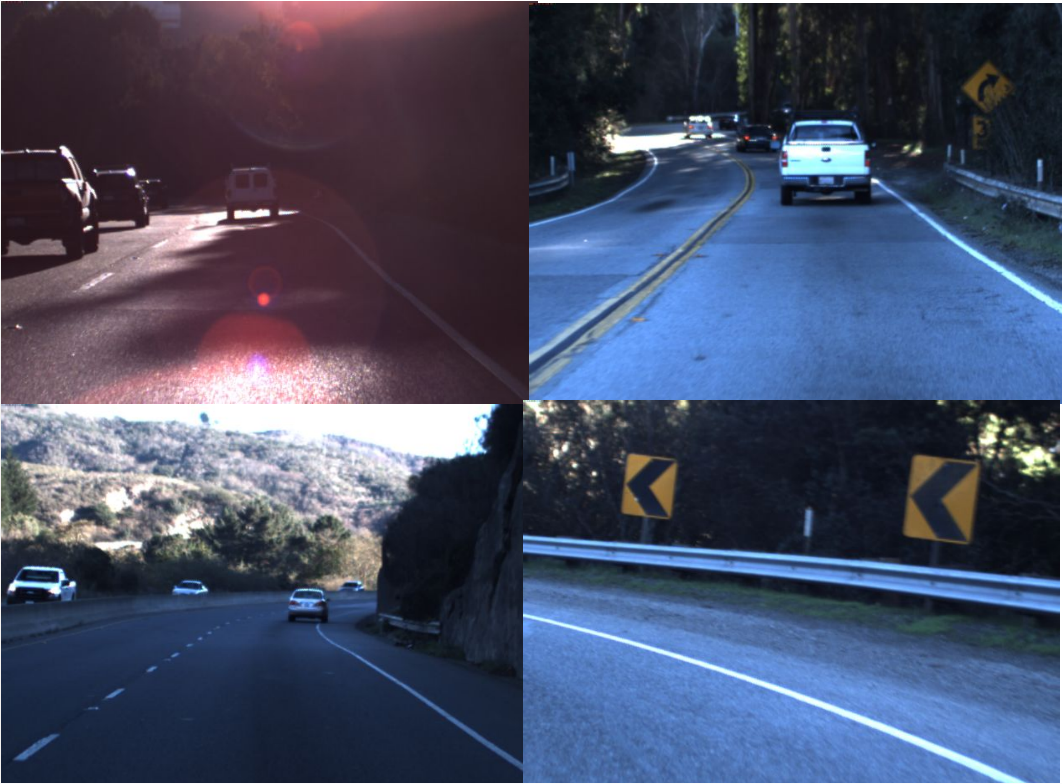
\includegraphics[scale=0.35]{steerdataset-samples}
	\caption{Sample images from the Udacity steering angle dataset. Image source: }
	\label{fig_steer_data_samples}
\end{figure}

Steering angle prediction is both a safety and time critical application which serves as an essential component of any autonomous vehicle. As enhancing functional safety in such applications is one of the key objectives of using uncertainty estimation methods, the steering angle data set is chosen for benchmarking the techniques considered for this research work.   
\subsection{Network architectures}
\subsubsection{Dronet}
Dronet, a residual convolutional network architecture is used for experiments conducted on the steering angle dataset. The Neural Network is primarily designed to safely navigate a drone by performing the tasks of steering angle prediction(regression) and collision detection(binary classification). However, for the experiments conducted in this research work the collision detection output is not required and therefore its corresponding output branch in the Neural Networks output layer is discarded. Figure \ref{fig_resnet8} depicts Dronet's architecture.

The model used for experiments takes a gray-scale input of size 200x200 and propagates it through a pair of convolution and max-pooling layers, three residual blocks, a dropout layer, a ReLU activation and finally a fully-connected(fc) layer which outputs predicted steering angles. When it comes to integrating MCDO\_ADF(described in \ref{general_framework}) with Dronet, new dropout layers are introduced before every convolutional layer at the test time. On the other hand, DER (described in \ref{der}) is integrated to Dronet by introducing three more output branches in the last fc layer for outputting parameters of the evidential distribution (described in \ref{sec_evidential_dist}).
\begin{figure}
	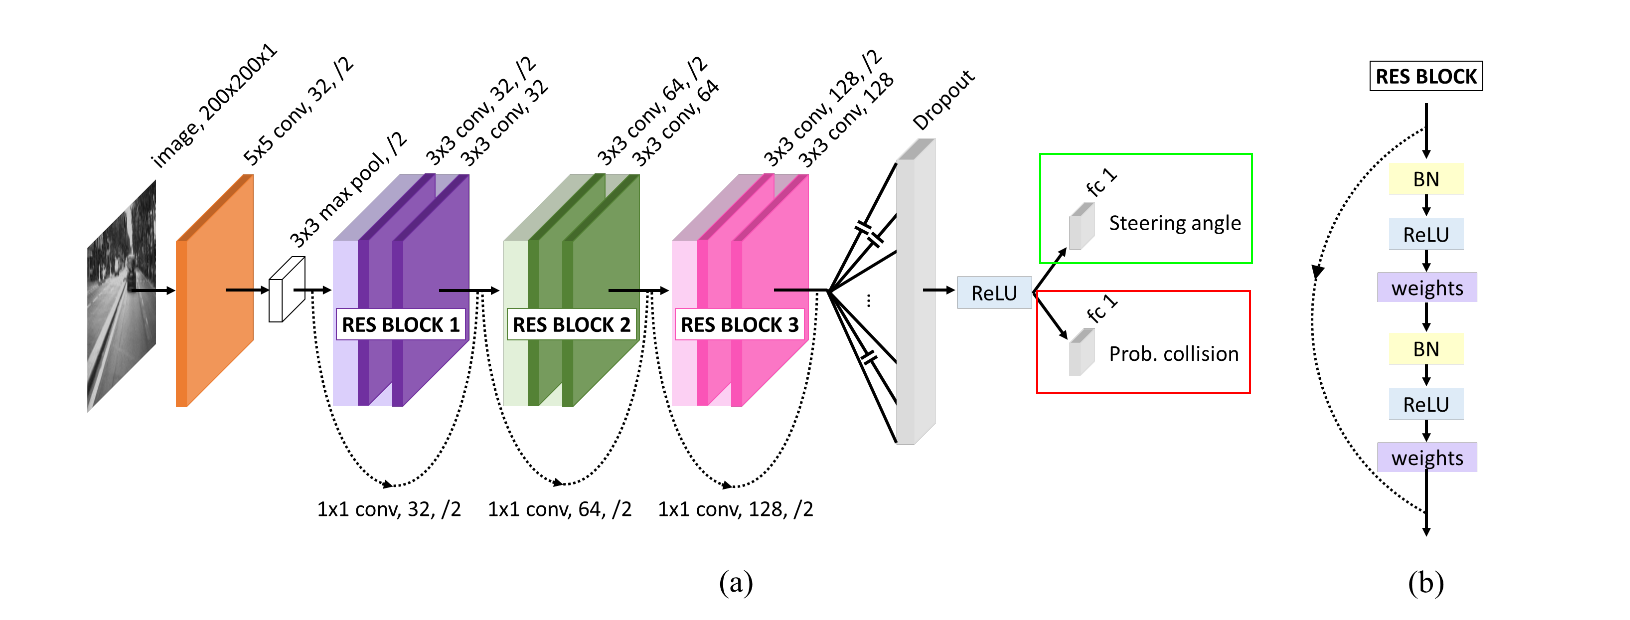
\includegraphics[scale=0.30]{resnet8}
	\caption{(a) Dronet architecture (b) Structure of every residual block . Collision classification output (bounded by the red box) is discarded and the steering angle prediction branch(bounded by the green box) is retained for this experiment.  Image source: }
	\label{fig_resnet8}
\end{figure}
 
\subsection{Training details}
\subsubsection{Dronet with steering angle dataset}
In order to benchmark the considered uncertainty estimation methods(MCDO\_ADF and DER), a set of three Dronet models are used: 1. Vanilla version of Dronet 2. MCDO\_ADF version of dronet with dropout layers after convolution layers 3. Evidential version of Dronet which uses the evidential loss function. Training details for those variants are provided in upcoming sections.

Choice of certain hyperparameter values remains unchanged for training all the three models and are listed in the table below.

\begin{table}[h]
	\centering
	\begin{tabular}{|l|l|}
		\hline
		\textbf{Hyperparameter} & \textbf{Value} \\ \hline
		Input image size (hxwxc)& 200 x 200 x 1  \\ \hline
		Batch size              & 32             \\ \hline
		Training epochs         & 100            \\ \hline
		Learning rate           & 0.001          \\ \hline
		Dropout rate            & 0.2            \\ \hline
		Weight decay            & 0.0001         \\ \hline
		Learning rate decay     & 0.00001        \\ \hline
		Choice of optimizer     & Adam           \\ \hline
	\end{tabular}
	\caption{List of hyperparameters with values remaining unchanged between training session of Dronet variants}	
\end{table}




\subsubsection{Vanilla Dronet}
A simple dronet model predicts steering angle for the given image input. Training the model involves reduction of the Mean Squared Error (MSE) loss, which is popular choice for regression problems. Optimizing the MSE loss function intuitively means reduction of mean over euclidean distance (L2-Norm) between ground truth labels and predictions of observed data. The MSE loss function can be expressed as follows:

\begin{equation}
	\mathbf{L}(y,\hat{y})=\frac{1}{N}\sum_{i=0}^{N}(y-\hat{y}_i)^2
\end{equation} 
\begin{figure}[h]
	\centering
	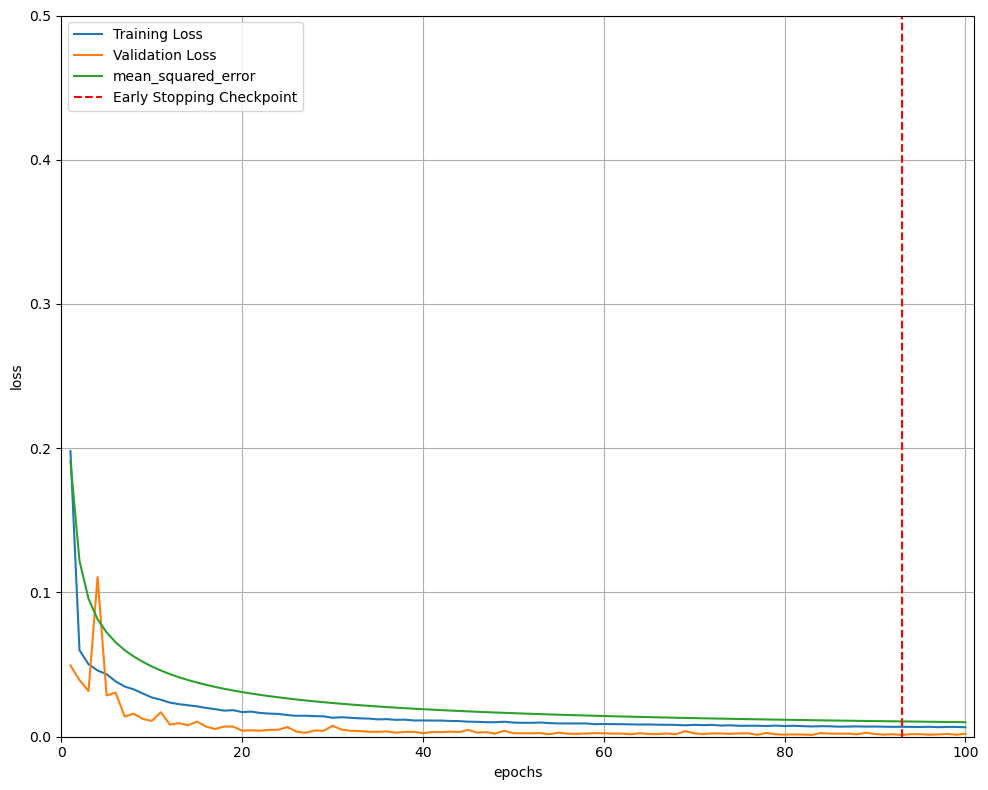
\includegraphics[scale=0.4]{dronet_mse_loss}
	\caption{Plot depicting the trend of Mean-Squared-Error loss while training vanilla Dronet}
	\label{fig_mse_loss_dronet}
\end{figure}

The technique of early stopping is used to avoid over-fitting, by saving model weights at the epoch corresponding to the least validation loss.

\subsubsection{MCDO\_ADF Dronet}
This variant of Dronet is trained to facilitate estimation of uncertainty associated with its predictions using the MCDO\_ADF technique. The training procedure for this variant remains unchanged from the Vanilla variant except for the  introduction of dropout after every convolution layer. Though it is sufficient to have the vanilla variant for applying this method, dropout was used during training with an intent to regularize the process.
\begin{figure}[h]
	\centering
	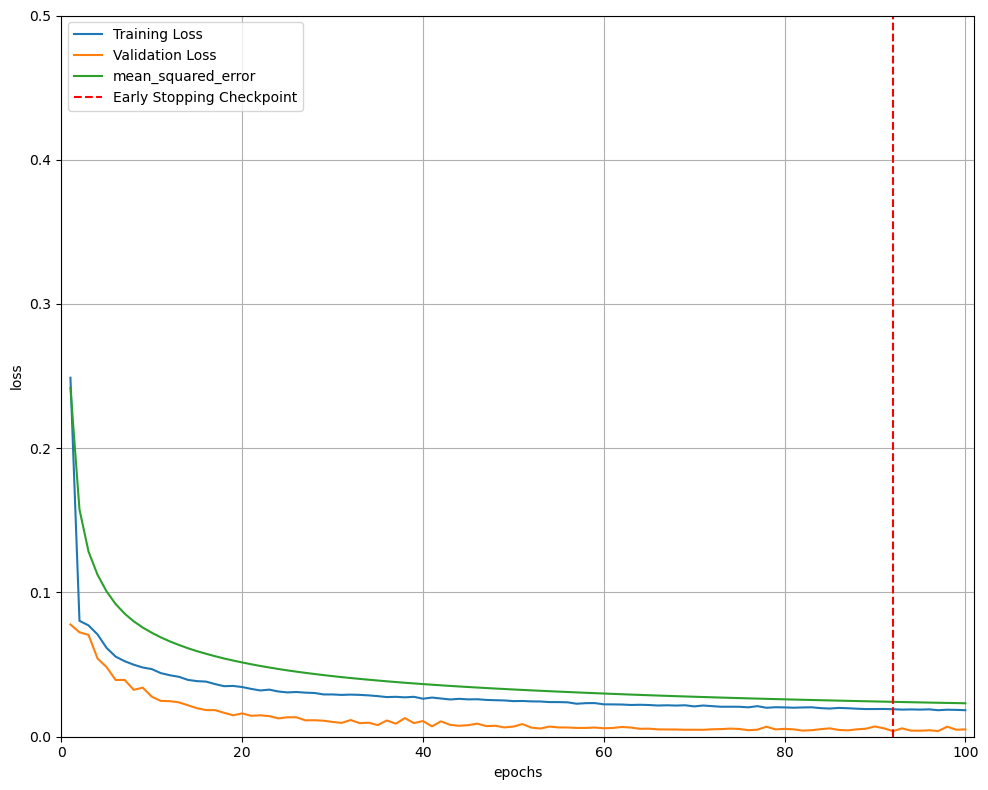
\includegraphics[scale=0.4]{dronet_MCDO_mse_loss_plot}
	\caption{Plot depicting the trend of Mean-Squared-Error loss while training MCDO\_ADF Dronet}
	\label{fig_mse_loss_mcdo_dronet}
\end{figure}

The inference procedure for MCDO\_ADF applied models is clearly explained in \ref{sec_mcdo_adf}. There are three hyper-parameters additionally required for the procedure: 1. Monte-Carlo(MC) sample count 2. Noise-variance 3. Minimum-variance. The value of MC sample count has a direct impact on the inference time as it determines number of forward passes for a given input to determine model uncertainty. For this experiment, we set its value to be 20 to replicate results provided in []. Both the values of noise-variance and minimum variance are chosen to be 0.001. Noise variance indicates the level of sensor noise and minimum-variance signifies the minimum value of noise-variance to be propagated through every layer.

\subsubsection{Evidential Dronet}
The evidential Dronet model outputs parameters of the evidential distribution(described in the section \ref{sec_evidential_dist}) for a given input image. The distribution parameters can be in turn used to calculate prediction and uncertainty associated with it. Except for the choice of evidential loss function(described in \ref{sec_evi_learning_objectives}) for this model , training criteria remains unchanged from the vanilla variant.
\begin{figure}[h!]
	\centering
	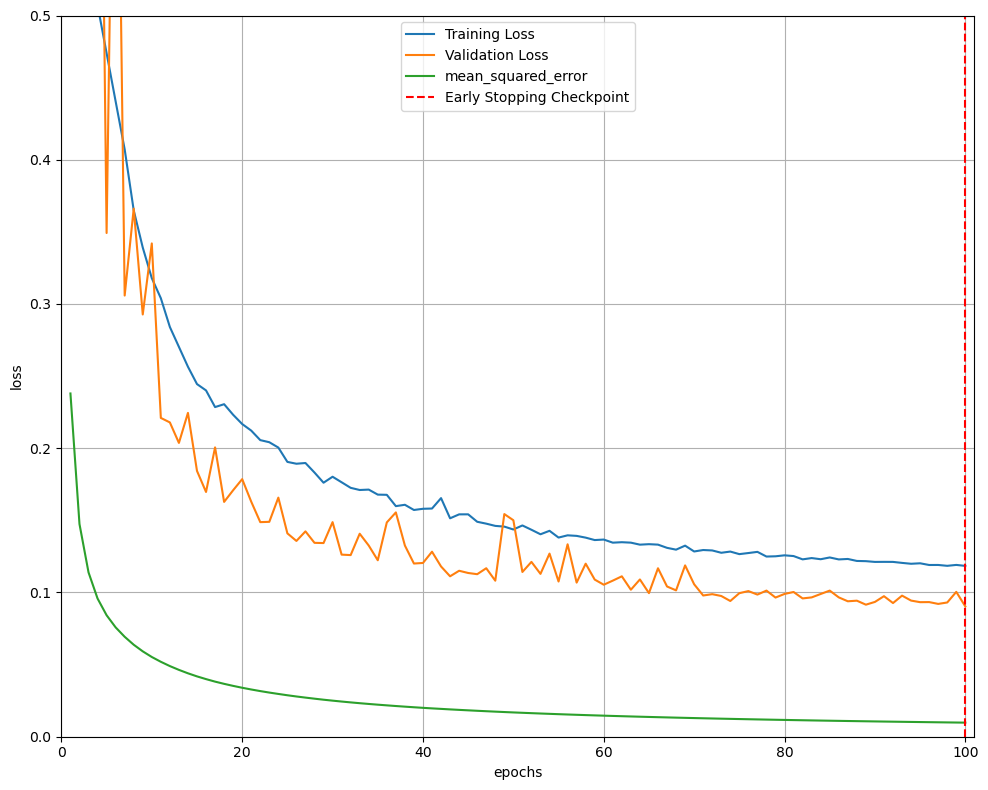
\includegraphics[scale=0.4]{dronet_evidential_loss_plot}
	\caption{Plot depicting the trend of evidential loss while training evidential Dronet}
	\label{fig_mse_loss_mcdo_dronet}
\end{figure}

\subsection{Metrics}
\subsubsection{Root Mean Squared Error(RMSE)}
Root Mean Squared Error (RMSE), measures the spread of distances between model predictions and their corresponding ground truth values. Alternatively, it can be explained as the standard deviation of prediction errors. RMSE is a well-known accuracy metric in regression problems. The metric is non-negative in nature with lower values indicating better model fit.
\begin{equation}
	\mathbf{RMSE} = \sqrt{\frac{\sum_{i=1}^{N}(\hat{y}_i-y_i)^2}{N}}
\end{equation}
Here $\hat{y}$,$y$ and $N$ represent ground truth labels, predictions and number of data points respectively.
\subsubsection{Explained Variance(EVA)}
The Explained Variance (EVA) is a measure of a regressor's ability to capture variance(variation) of given data. The metric can be computed with the following expression:
\begin{equation}
	\mathbf{EVA} = \frac{Variance(\hat{y}-y)}{Variance(\hat{y})}
\end{equation}
Here $\hat{y}$,$y$ represent ground-truth labels and predictions respectively. The numerator term denotes variance of residuals whereas the denominator denotes the underlying variance in ground-truth labels. For an ideal regressor, the value of EVA equals 0.
\subsubsection{Negative-Log-Likelihood(NLL)}
In this research work,the Negative-Log-Likelihood(NLL) metric is used compare performance of uncertainty estimation methods. NLL for a given pair of prediction and uncertainty can be computed as follows
\begin{itemize}
	\item A distribution (often Gaussian) is created with the model prediction as its mean and uncertainty as its variance.
	\item The conditional probability of observing the ground-truth label(corresponding to the input) in the created distribution is determined. This is nothing but the likelihood value of ground-truth in the created distribution.
	\item  In order to handle and effectively represent very low values of likelihood, negative of natural logarithm is applied  to the value. After application of negative logarithm, the total likelihood can be computed by summing all individual values.
\end{itemize}
\begin{equation}
	\mathbf{NLL} = -\sum_{i=1}^{N}\ln P(\hat{y}_i|\mathcal{N}(y_i,\sigma^2)) 
\end{equation}
Here $\hat{y}$,$y$,$\sigma^2$ and $N$ represent ground truth labels, predictions, predictive uncertainty and number of data points respectively.
Lower the value of NLL better the performance of an uncertainty estimation method associated with it. However, the value of NLL highly depends on the number and choice of test points used for evaluation. Therefore, the metric can be used to compare performance of uncertainty estimation methods only when the same data set is used for their evaluation.
\subsection{Quantitative comparison}
\begin{table}[h!]
	\centering
	\begin{tabular}{|c|c|c|c|c|c|}
		\hline
		\multirow{2}{*}{\textbf{Model}} & \multirow{2}{*}{\textbf{RMSE}} & \multirow{2}{*}{\textbf{EVA}} & \multicolumn{3}{c|}{\textbf{NLL}}                             \\ \cline{4-6} 
		&                                &                               & \textbf{Epistemic} & \textbf{Aleatoric} & \textbf{Predictive} \\ \hline
		Vanilla Dronet                  & 0.034                          & 0.98                          & NA                 & NA                 & NA                  \\ \hline
		MCDO\_ADF Dronet                & 0.15                           & 0.68                          & -0.71              & 7.51               & -0.74               \\ \hline
		Evidential Dronet               & \textbf{0.022}                 & \textbf{0.99}                 & \textbf{-2.03}     & \textbf{-1}        & \textbf{-0.94}      \\ \hline
	\end{tabular}
\caption{A quantitative comparison of uncertainty estimation methods when applied to Dronet}
\label{tab_quant_compare}
\end{table}
\begin{itemize}
	\item It can be inferred that Evidential Dronet outperforms the other two models in terms of both predictive accuracy and quality of uncertainty estimation.
	\item In the case of predictive accuracy expressed in terms of RMSE, Evidential Dronet outperforms the Vanilla variant only by a slight margin. However, difference in RMSE between Evidential and MCDO\_ADF variants is considerable. This could be partly attributed to the fact that both predictions and uncertainty estimates outputted by the MCDO\_ADF variant depend on the count of Monte-Carlo(MC) samples considered. Higher the value of MC samples better the model's performance(refer figure \ref{fig_mc_count_vs_rmse}).  However, this holds true only un till a particular value of MC samples. For this experiment, 20 MC samples are considered. 
	\item The relationship between MC sample counts and predictive accuracy holds good for the Explained Variance (EVA) measure as well.
	\item The quality of predictive uncertainty estimated by the Evidential Dronet expressed in terms of Negative-Log-Likelihood (NLL) is better than the MCDO\_ADF variant. This intuitively means that the former technique is able to determine parameters of the distribution in which likelihood of finding ground truth labels is higher than in the distribution outputted by the latter.
\end{itemize}
\begin{figure}[h]
	\centering
	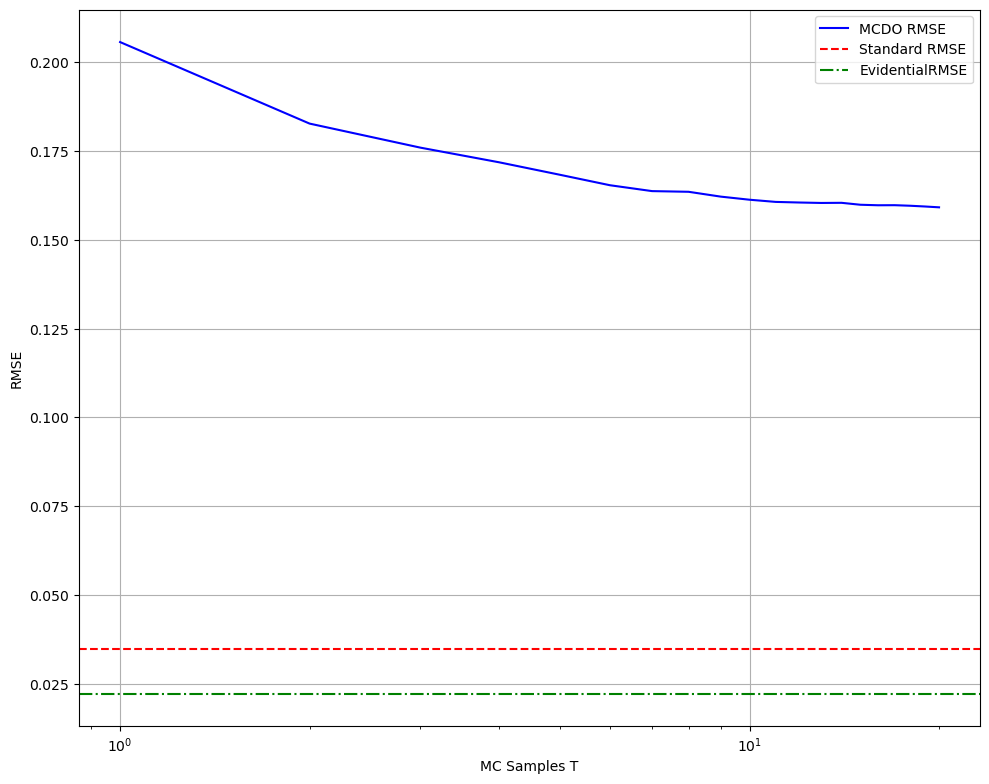
\includegraphics[scale=0.5]{RMSE_T20}
	\caption{A plot depicting relationship between the MC sample count and RMSE during the MCDO\_ADF model inference}
	\label{fig_mc_count_vs_rmse}
\end{figure}
\subsection{Qualitative comparison}
In order to qualitatively compare predictive uncertainties outputted by both the models, test images corresponding to the highest and lowest values of uncertainty(aleatoric, epistemic and predictive) are taken into consideration and analyzed. For the analysis presented below, the set of images corresponding to an extreme value of uncertainty estimated by a method is represented in the form of "extreme\_category\_method". For example, images corresponding to high values of aleatoric uncertainty estimated by MCDO\_ADF is represented as "high\_aleatoric\_adf". The analysis is presented in form of a table.  
\end{document}
